\clearpage
\section{Interface}
\label{sec:interface}

This section has some examples of what the web user interface could look like.
At the time of writing, the numbers in these mock-ups agree with the content of \texttt{practice\_data/}.

\begin{figure}[h]
    \begin{minipage}[c]{0.23\textwidth}
        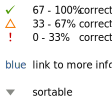
\includegraphics[width=\textwidth]{images/legend}
    \end{minipage} \hfill
    \begin{minipage}[c]{0.72\textwidth}
        \caption{Graphical elements of the user interface.
            (i) Performance is reported as the proportion of items on which the correct result was obtained.
            The checkmark, triangle, and exclamation marks are quick visual indicators of whether results were good, cautionary, or bad.
            (ii) Text in a blue font is a link to a page that contains more information.
            (iii) Arrows in the header of a table indicate that the table can be sorted by that column.
            Sorting should be iterative, e.g., sort first on the contents of one column (click its arrow), and then within each of those categories sort based on a second column (shift-click its arrow).
        }
        \label{fig:ui_legend}
    \end{minipage}
\end{figure}

%--------------------------------------------------
\subsection{Overview of how all methods perform}
%--------------------------------------------------

The highest-level display of results summarizes the performance of each \Method on each \Benchmark for a given \Task (\cref{fig:ui_methods_benchmarks}).
The goal is give a quick visual summary of which \Methods do well, and which \Benchmarks are challenging.

\begin{figure}[h]
    \centering 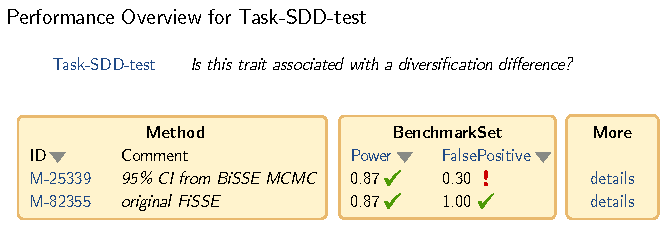
\includegraphics[width=0.8\textwidth]{images/methods_benchmarks}
    \caption{Performance of all \Methods for a \Task.
        Each number is the average of the \Method's success for each \Element in that \Benchmark.
        The `details' link leads to a view like \cref{fig:ui_method_performance}.
        The links from each model (in the `ID' column), each \Benchmark (`Power', `FalsePositive'), and the \Task (`Task-SDD-test') each lead to a page displaying all the information for that component (details, scripts, contributor information, etc.).
    }
    \label{fig:ui_methods_benchmarks}
\end{figure}

%--------------------------------------------------
\subsection{Performance of one method}
%--------------------------------------------------

Focusing on a single \Method, we can see in more detail how it performs across all the \Elements that comprise the \Benchmarks (\cref{fig:ui_method_performance}).

\begin{figure}[h]
    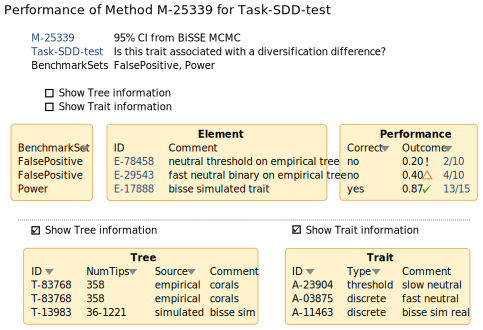
\includegraphics[width=0.9\textwidth]{images/method_performance}
    \caption{Performance of one \Method for all relevant \Benchmarks.
        Each number is the proportion of datasets (tree-trait combinations) in an \Element on which the \Method gave the `Correct' answer.
        (This column header might be confusing, but I mean that the correct answer to the \Task's question is `no' for the first \Element, etc.)
        The numerical links (`2/10' etc.) lead to a more detailed report of the results.
        The checkboxes allow the user to specify whether more information about the \Tree and/or \Trait in each \Element should be displayed.
        If a box is checked, further columns are displayed in the table (to the right of `Performance'), as illustrated below the dotted line.
    }
    \label{fig:ui_method_performance}
\end{figure}
